Las estrellas de neutrones son sistemas astronómicos con nucleones sometidos a condiciones extremas.
Debido a la combinación entre la atracción nuclear y la repulsión de Coulomb entre protones el sistema tiene inhomogeneidades en su estructura.
Estas inhomogeneidades aparecen también en sistemas expandiéndose, donde la distribución de fragmentos depende de las condiciones termodinámicas (temperatura, fracción de protones, \ldots) y la velocidad de expansión.

El origen de elementos pesados (más pesados que el $^{56}_{26}\text{Fe}$) es aún una incógnita en la física.
Las principales hipótesis respecto del origen de estos elementos implican que las colisiones de estrellas de neutrones serían responsables de más de la mitad de la abundancia terrestre.
El reciente descubrimiento de colisiones de estrellas de neutrones y sus correspondientes ondas gravitacionales~\cite{ligo_scientific_collaboration_and_virgo_collaboration_gw170817_GW170817:_2017} en LIGO representa la primera oportunidad para detectar y estudiar el impacto de éstas.
Recientes trabajos~\cite{kasen_origin_2017} han estudiado, mediante modelos hidrodinámicos, el rol de las colisiones de estrellas de neutrones en la generación de elementos pesados.
Al producirse la colisión de dos estrellas de neutrones, la materia se fragmenta en condiciones extremas.
Estas condiciones, de acuerdo a Ref.~\cite{lattimer_black-hole-neutron-star_1974}, son favorables para que se produzca el \emph{r-process} y, en conclusión, una fuente posible para núcleos terrestres.
Inspirados por la colisión de estrellas de neutrones, desarrollamos un estudio en la fragmentación de materia de estrellas de neutrones en expansión.

El objetivo es encontrar la dinámica de la formación de los fragmentos para sistemas que se expanden de acuerdo al modelo del pequeño \emph{big bang}~\cite{dorso_onset_1996}.
Esta expansión se parece a la evolución de las colisiones de estrellas de neutrones.
A partir de una configuración de equilibrio, expandimos el sistema homogéneamente hasta llegar a una configuración asintótica (i.\ e.\ densidades muy bajas).
Estudiamos, con cuatro algoritmos reconocedores de fragmentos distintos, la distribución de fragmentos a lo largo de esta expansión y la dinámica de la formación de fragmentos.

Encontramos los típicos regímenes de la distribución de fragmentos de una expansión: U-shaped, ley de potencias y exponencial.
Otra característica de nuestro cálculo es que, ya que la interacción entre protones es repulsiva de largo rango, no siempre tenemos un fragmento infinito.
Como es de esperar, cuanto más rápida es la velocidad e expansión, más rápido desaparece el fragmento infinito.

Desarrollamos una herramienta basada en análisis de grafos para la identificación del fragmento infinito y encontramos una transición de distribución de fragmentos de U-shaped a exponencial a medida que aumenta la velocidad de expansión.

Estudiando la topología de los estados de equilibrio, antes de la expansión, reprodujimos las pastas usuales y, además, una nueva fase que hemos llamado \emph{pregnocchi}, que consiste de agregados de protones embebidos en un  \emph{mar de neutrones}.
Identificamos distintos regímenes de fragmentación, dependiendo de la temperatura inicial y la velocidad de expansión.
En particular, para los ya mencionados \emph{pregnocchi}, una nube de neutrones rodea a los fragmentos a lo largo de los comienzos de la expansión, resultando en sistemas con configuraciones compatibles con la emergencia del \emph{r-process}.

Mostramos que una identificación adecuada de la distribución de fragmentos depende del algoritmo de reconocimiento de fragmentos escogido, y que el Algoritmo de Reconocimiento Temprano de Fragmentos (ECRA) fue el más estable.
Este enfoque nos permitió identificar la dinámica de la formación de fragmentos.
Estos cálculos pueden ser el comienzo de una comparación entre los experimentos de fragmentación terrestres y los estudios de estrellas de neutrones.

\section{Introducción}
En configuraciones típicas tenemos no sólo la estructura conocida como pasta nuclear, sino también, para ciertos valores de la fracción de protones $x$, un gas de nucleones en que aquélla está embebida.
Para caracterizar adecuadamente las fases de pasta debemos saber cuáles partículas pertenecen a las fases de pasta y cuáles al gas.
Así, lo que debemos es encontrar los fragmentos que se forman a lo largo de la simulación.

Uno de los algoritmos para identificar la formación de fragmentos es el conocido como Minimum Spanning Tree (MST).
En el algoritmo MST dos partículas pertenecen al mismo cluster $\{C^{\text{MST}}_n\}$ si la distancia entre ellas es menor que una distancia de corte $r_{cut}$:
\begin{equation*}
  i \in C^{\text{MST}}_n \Leftrightarrow \exists j \in C_n \mid
  r_{ij} < r_{cut}
\end{equation*}

Esta definición de fragmentos funciona adecuadamente para sistemas sin energía cinética y baja densidad (en general, sistemas fríos y diluidos), y está basada en la cola atractiva de la interacción nuclear.
Sin embargo, si el sistema tiene una temperatura mayor a cero, podemos tener una situación en la que dos partículas están más cerca que la distancia de corte, pero con una energía cinética relativa tan grande que van a separarse indefectiblemente.

Para tratar situaciones de temperatura mayores a cero, tenemos que tener en cuenta el momento relativo entre las partículas.
Uno de los métodos mas sofisticados para lograr esto es el Algoritmo de Reconocimiento Temprano de Fragmentos~\cite{dorso_early_1993}.
En este algoritmo, las partículas se particionan en distintos fragmentos disjuntos, $C^{\text{ECRA}}_n$, con la energía total para cada fragmento:
\begin{equation*}
  \epsilon_n = \sum_{i \in C_n} K^{CM}_i +  \sum_{i,j \in C_n} V_{ij}
\end{equation*}
donde $K^{CM}_i$ es la energía cinética relativa al centro de masa del fragmento.
El conjunto de fragmentos $\{C_n\}$ es, entonces, el que minimiza la suma de todas las energías de los fragmentos $E_{\text{partición}} =
\sum_n \epsilon_n$.

El algoritmo ECRA puede ser utilizado fácilmente para sistemas pequeños~\cite{dorso_fluctuation_1994}, pero al ser una optimización combinatoria, no puede ser utilizado en sistemas grandes.
Mientras que encontrar fragmentos ECRA es muy costoso computacionalmente, utilizar simplemente fragmentos MST resulta en fragmentos excesivamente grandes.
Una alternativa es el algoritmo Minimum Spanning Tree Energy (MSTE)~\cite{dorso_topological_2012}.
Este algoritmo es una modificación de MST, considerando la energía cinética.
De acuerdo a este algoritmo, dos partículas pertenecen al mismo fragmento $\{C^{\text{MSTE}}_n\}$ si están unidas energéticamente:
\begin{equation*}
  i \in C^{\text{MSTE}}_n \Leftrightarrow \exists j \in C_n :
  V_{ij}+ K_{ij} \le 0
\end{equation*}
A pesar de que de este algoritmo no se obtienen los mismos resultados teóricamente consistentes que con ECRA, igual evita el mayor problema de MST: no considerar de ninguna manera la energía cinética.

\subsection{Identificación de Fragmentos Infinitos}
Desarrollmos un algoritmo para el reconocimiento de fragmentos infinitos a través de los contornos.
Explicamos aquí en detalle la implementación para fragmentos tipo MST en 2 dimensiones, mientras que la extensión a MSTE y 3 dimensiones es inmediata y, en general, a cualquier definición de clusters que cumpla con la \emph{aditividad}.
En la figura~\ref{fig:scheme_clusters} podemos ver una representación esquemática de fragmentos 2D reconocidos en una celda periódica, etiquetados del 1 al 6 (notar que estos fragmentos no se conectan aún a través de las paredes periódicas).

\begin{figure}  \centering
  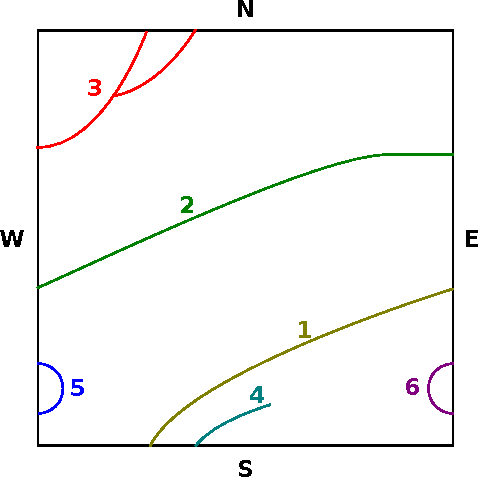
\includegraphics[width=0.75\columnwidth]{fragmentacion/scheme_clusters}
  \caption{Representación esquemática de fragmentos 2D, reconocidos sólo en la celda y no a través de las paredes periódicas, etiquetadas como N, S, W y E.
  Los fragmentos dentro de la celda están etiquetados del 1 al 6.}
\label{fig:scheme_clusters}
\end{figure}

Para hallar las conexiones entre estos fragmentos a través de los contornos, dibujamos un grafo de los fragmentos, donde los conectamos dependiendo de si se conectan o no a través de una pared, y etiquetamos dicha conexión con la etiqueta de la pared.
Por ejemplo, comenzamos con el fragmento 1.
Se conecta con el fragmento 2 a través de la pared E, por lo que agregamos una conexión $1\rightarrow2$ etiquetada como E.
Simétricamente, agregamos una conexión $2\rightarrow1$ etiquetada W.
Ahora vamos por el par 1-3.
Se conecta a través de la pared S, por lo que agregamos $1\rightarrow3$ con la etiqueta S y $3\rightarrow1$ con la etiqueta N.
El fragmento 1 no se conecta con los 4, 5 o 6, por lo que éstas son las únicas conexiones que tenemos para dicho fragmento.
Una vez que hayamos hecho eso, obtenemos el grafo de la figura~\ref{fig:graph_clusters}.

\begin{figure}  \centering
  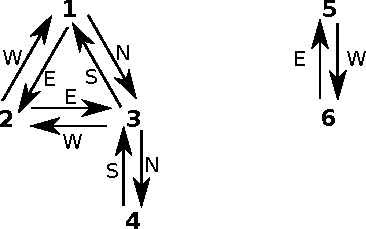
\includegraphics[width=0.45\columnwidth]{fragmentacion/graph_clusters}
  \caption{Grafo de los fragmentos con conexiones etiquetadas por la etiqueta de la pared a través de la cual se conectan.
    El grafo puede ser dividido en dos subgrafos que no se conectan entre ellos: 1--2--3--4 y 5--6.
    Cada uno de estos subgrafos es un fragmento al considerar las condiciones periódicas de contorno.}
\label{fig:graph_clusters}
\end{figure}

Ahora nos preguntamos si estos subgrafos representan un fragmento infinito o no.
Para tener un fragmento infinito necesitamos un ciclo cerrado (lo opuesto no es cierto: tener un circuito cerrado no es suficiente para tener un fragmento infinito, como podemos ver en el subgrafo 5--6), de modo que primero identificamos ciclos y los marcamos como candidatos para fragmentos infinitos.
Cada conexión agrega un ciclo (ya que las conexiones de los fragmentos son ida y vuelta), pero sabemos de inspeccionar la figura~\ref{fig:graph_clusters} que el fragmento 1--2--3 es infinito.
La clave para identificar en los grafos los fragmentos infinitos es identificar, en el grafo, qué hace al fragmento 1--2--3 infinito.
La característica fundamental del fragmento 1--2--3 es que su ciclo 1--2--3--1 puede ser circulado a través de las paredes E--E--S, mientras que el 5--6 puede ser circulado sólo a través de E--W.
Ahora, para que el fragmento sea infinito, necesitamos que se extienda infinitamente en, al menos, una dirección.
De este modo, una vez que tenemos la lista de paredes del ciclo, creamos una magnitud $I$ asociada a cada ciclo, que se crea de la siguiente manera.
Comenzando con $I=0$, agregamos un valor $M_i$ si hay al menos una pared de tipo $i$.
Los valores son: $M_E= 1$, $M_W = -1$, $M_N = 2$, $M_S = -2$.
Si $I$ no es cero, entonces el ciclo es infinito.
Por ejemplo, el ciclo  E--E--S tiene paredes E y S, de modo que $I = M_E + M_S = -1$ y el ciclo es infinito.
Para el ciclo E--W, $I = M_E + M_W = 0$, y el ciclo es finito.

\section{Expansión}\label{sc:expansion}
La simulación de la colisión de dos estrellas de neutrones es impracticable computacionalmente con este nivel de detalle, ya que implicaría resolver aproximadamente $10^{30}$ veces la celda de simulación que utilizamos.
En vez de simular la colisión de las estrellas, emulamos su comportamiento realizando expansiones locales de sistemas infinitos.
Para expandir la materia rica en neutrones que simula un sistema infinito con condiciones periódicas de contorno, seguimos el método del \emph{big bang microscópico}, explicado por Holian y Grady en Ref.~\cite{holian_fragmentation_1988} y usado por la expansión de sistemas infinitos previamente~\cite{dorso_onset_1996}.
Consiste en una expansión de la celda de simulación a un ritmo isotrópico y constante $\dot{\eta}$:
\begin{equation}
  L(t) = L_0\,(1+\dot{\eta}\,t)
\end{equation}
donde $L$ es la longitud inicial de la celda de simulación en cada dirección y $L_0$ es la longitud inicial.
Sólo con esta modificación del tamaño de la caja, el sistema se expandiría dinámicamente.
Para simular una expansión, necesitamos también que las partículas tengan una velocidad radial extra que concuerde con la de la celda en los bordes de la simulación:
\begin{equation}
  \mathbf{v} = \mathbf{v_0} + \dot{\eta}\,\mathbf{r_0}
\end{equation}

Ya que estamos trabajando con condiciones periódicas de contorno, cuando una partícula cruza un contorno, debemos considerar la expansión original, por lo que no cambiamos sólo la posición de la partícula sino también la velocidad.
Por ejemplo, si la partícula cruza el contorno izquierdo de la caja periódica, la velocidad de la partícula imagen $v_i^\dagger$ en el lado derecho debe ser modificada $v_i^\dagger = v_i + L_0\,\dot{\eta}$.
Esta prescripción para la expansión es matemáticamente equivalente a la ley de Hubble en astrofísica~\cite{chikazumi_quantum_2001}.
Es interesante notar que la expansión con esta prescripción es (para el sistema infinito simulado) adiabática: del momento inicial en adelante, no se agrega más energía al sistema.

\section{Fragmento infinito}
En la figura~\ref{fig:morpho} mostramos los estados inicial y final de la expansión de la celda principal de $N=11000$ partículas para velocidades de expansión muy bajas.
Podemos ver que, más allá de que la configuración inicial muestra una distribución de partículas compacta, la configuración final consiste de \emph{gnocchi} (casi esféricos) con una masa de alrededor de 80 partículas.

\begin{figure} \centering
  \begin{subfigure}[h!]{0.45\columnwidth}
    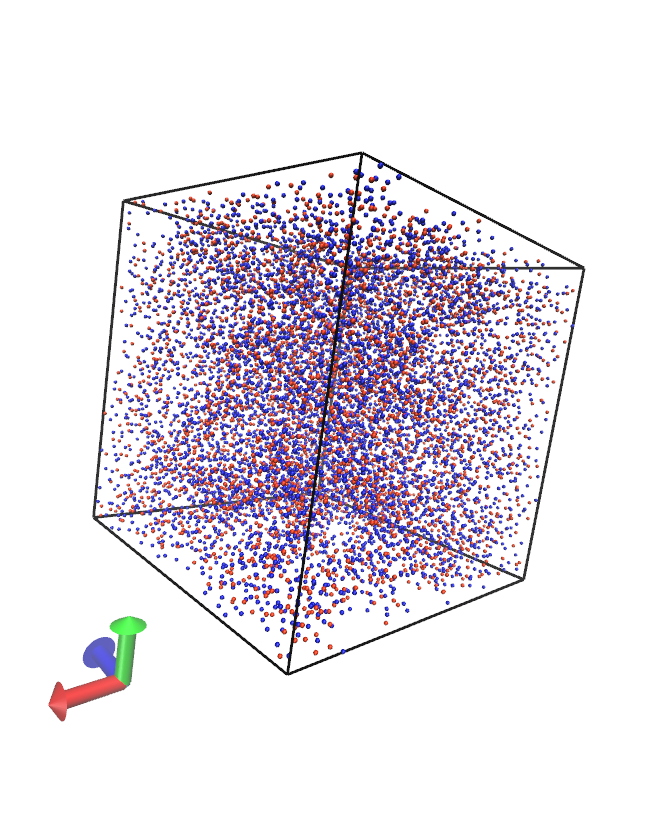
\includegraphics[width=\columnwidth]{fragmentacion/initial}
    \caption{$\eta = 0.0001\,\text{fm/c}$}
    \label{subfig:initial}
  \end{subfigure}
  \begin{subfigure}[h!]{0.45\columnwidth}
    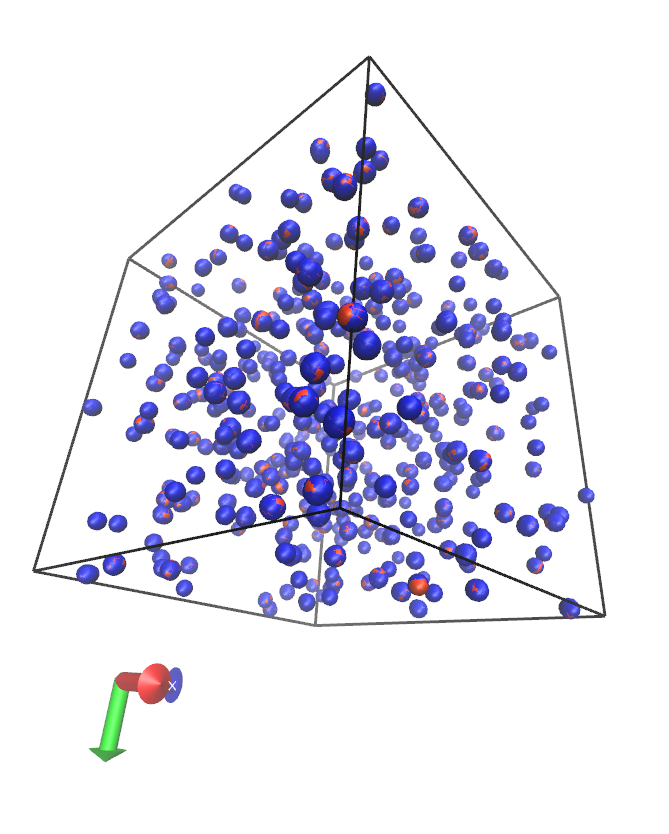
\includegraphics[width=\columnwidth]{fragmentacion/expanded}
    \caption{$\eta = 0.0005\,\text{fm/c}$}
    \label{subfig:expanded}
  \end{subfigure}
  \caption{Estructuras de un sistema en su configuración inicial~\ref{subfig:initial} y el sistema expandido final~\ref{subfig:expanded}.
    En el sistema expandido podemos ver que se forman fragmentos de tipo \emph{gnocchi}.}
  \label{fig:morpho}
\end{figure}

En la figura~\ref{fig:infinite} mostramos la fracción de partículas en la celda principal que forman parte de un cluster infinito (\emph{Fracción de Fragmento Infinito}, FFI).
Podemos ver fácilmente que en las primeras etapas de la evolución, como la temperatura es baja, la mayor parte del sistema en la celda principal pertenece al fragmento infinito.
Sin embargo, a medida que evoluciona el sistema de acuerdo a la velocidad de expansión, la FFI disminuye y llega a cero rápidamente, implicando que no hay fragmentos infinitos en el sistema.

\begin{figure}
  \centering
  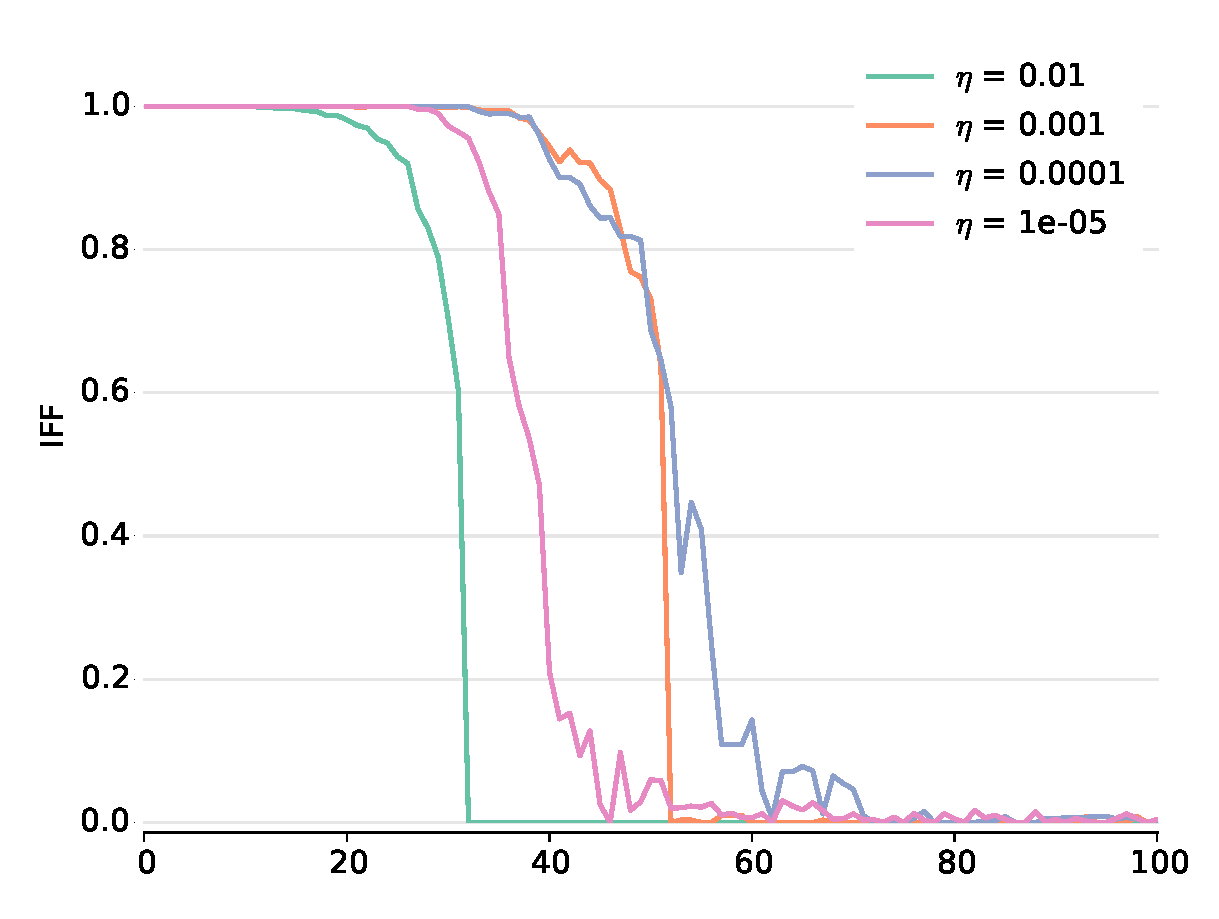
\includegraphics[width=0.75\columnwidth]{fragmentacion/infinite.pdf}
  \caption{Fracción de Fragmento Infinito (ver texto) en función de la longitud de la celda principal.
    Para todas las velocidades de expansión mostradas el FFI va a cero en el régimen asintótico.}
  \label{fig:infinite}
\end{figure}

\section{Fragmentos asintóticos}

La figura~\ref{fig:distribution} muestra la distribución de fragmentos asintóticos para cuatro distintas velocidades de expansión.
En este caso, el algoritmo MSTE fue aplicado sobre la celda principal, considerando las condiciones periódicas de contorno y sabiendo que no hay fragmento infinito, como se ve de la figura~\ref{fig:infinite}.
Podemos ver que a medida que aumenta la velocidad de expansión, la distribución de fragmentos muestra la típica transición de U-shaped a decaimiento exponencial.
Entre estas dos, aparece una distribución de tipo ley de potencias.
En particular, la figura~\ref{subfig:9e-3} muestra que con una expansión de $\eta = 0.009\,\text{fm/c}$ obtenemos una ley de potencias.
Es interesante notar que a diferencia de casos típicos de estudios de fragmentos, como percolación o sistemas de Lennard-Jones, debido a la presencia del término de repulsión de Coulomb, no es posible ver un fragmento infinito en el régimen asintótico.

\begin{figure} \centering
  \begin{subfigure}[h!]{0.45\columnwidth}
    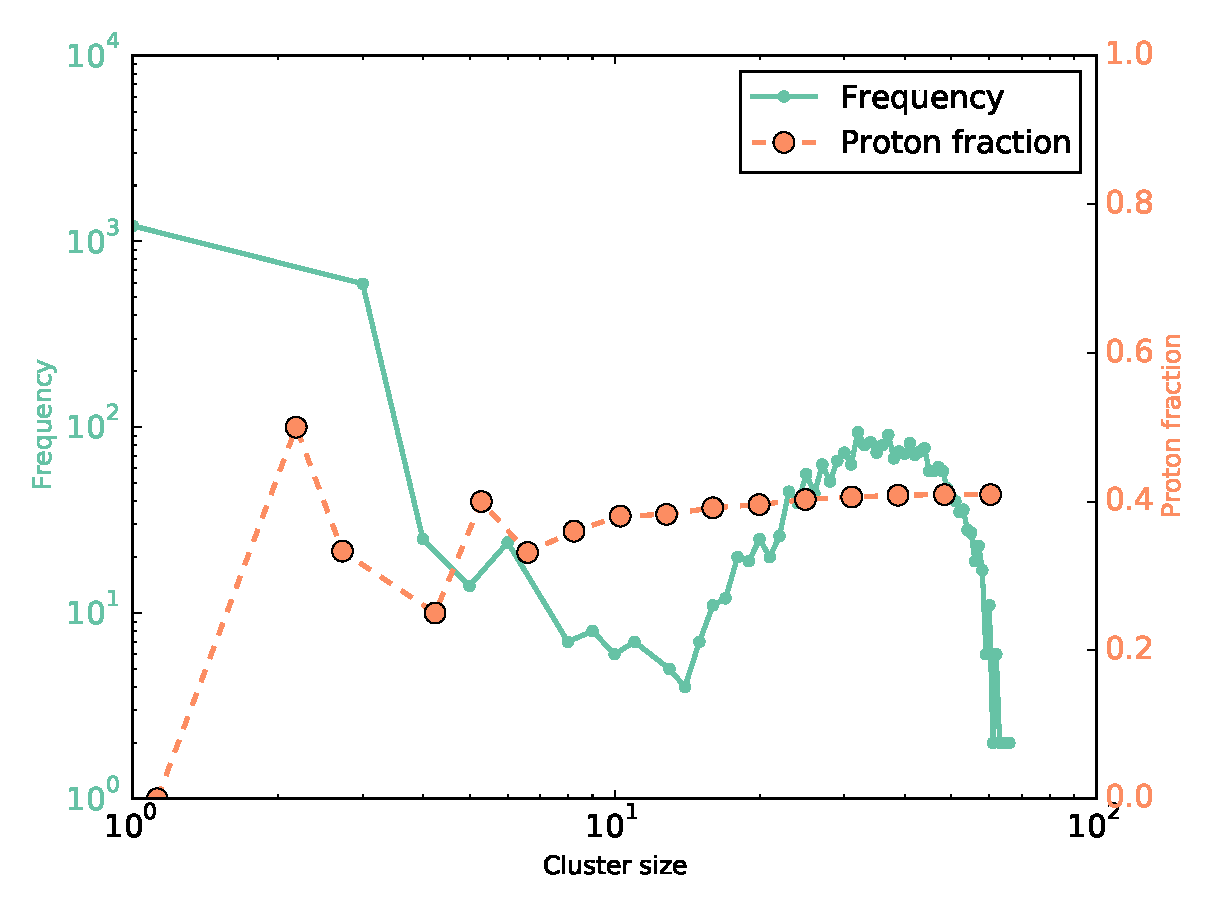
\includegraphics[width=\columnwidth]{fragmentacion/cluster_1e-4}
    \caption{$\eta = 0.0001\,\text{fm/c}$}
    \label{subfig:1e-4}
  \end{subfigure}
  \begin{subfigure}[h!]{0.45\columnwidth}
    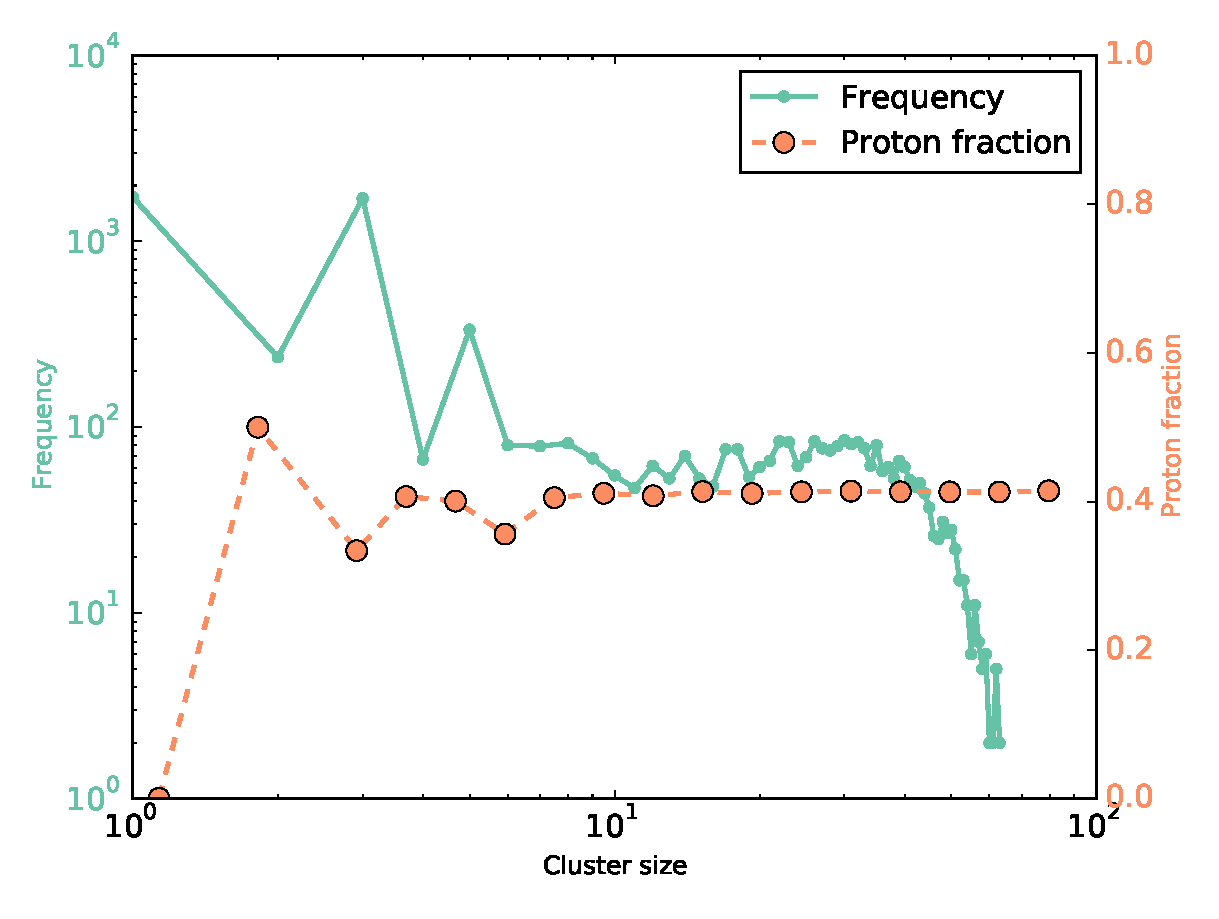
\includegraphics[width=\columnwidth]{fragmentacion/cluster_5e-4}
    \caption{$\eta = 0.0005\,\text{fm/c}$}
    \label{subfig:5e-4}
  \end{subfigure}
  \begin{subfigure}[h!]{0.45\columnwidth}
    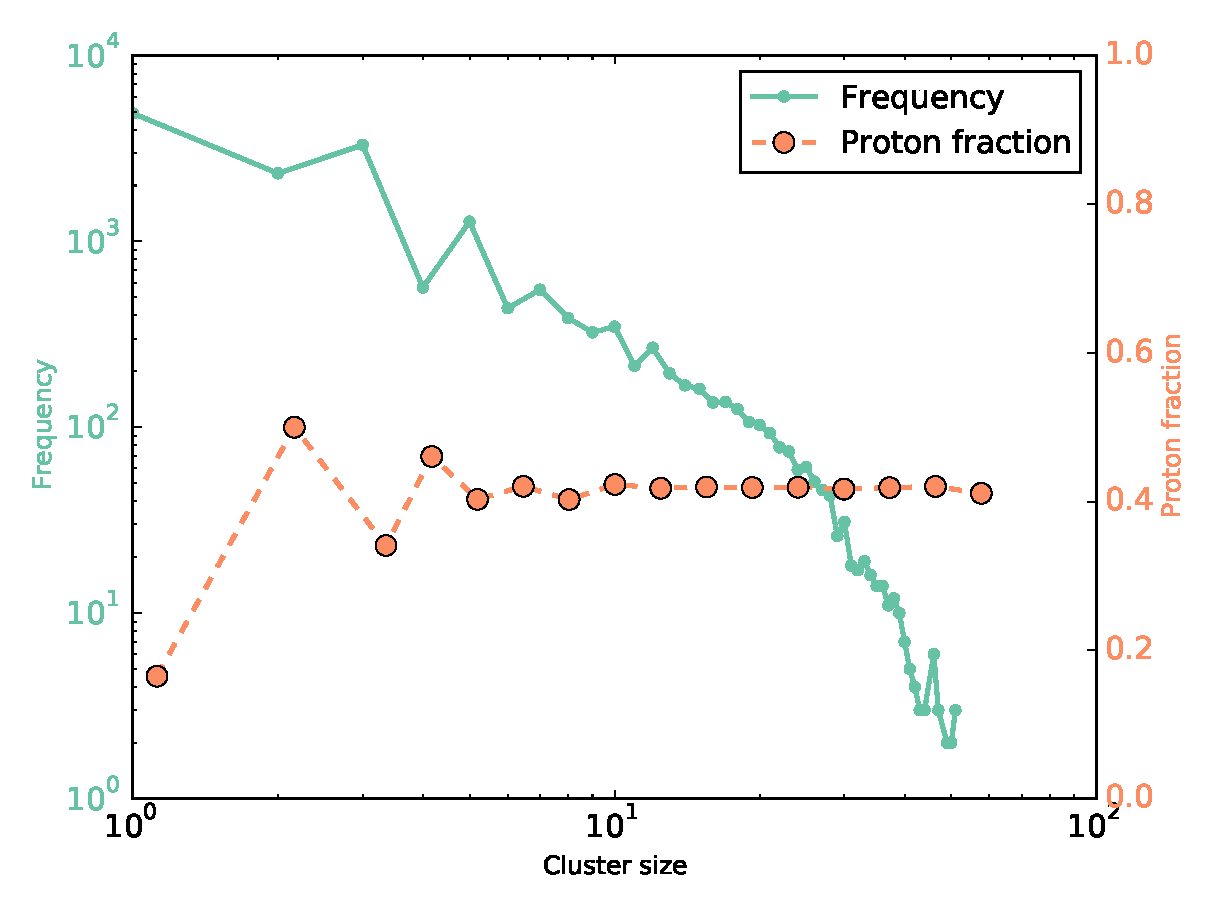
\includegraphics[width=\columnwidth]{fragmentacion/cluster_9e-3}
    \caption{$\eta = 0.009\,\text{fm/c}$}
    \label{subfig:9e-3}
  \end{subfigure}
  \begin{subfigure}[h!]{0.45\columnwidth}
    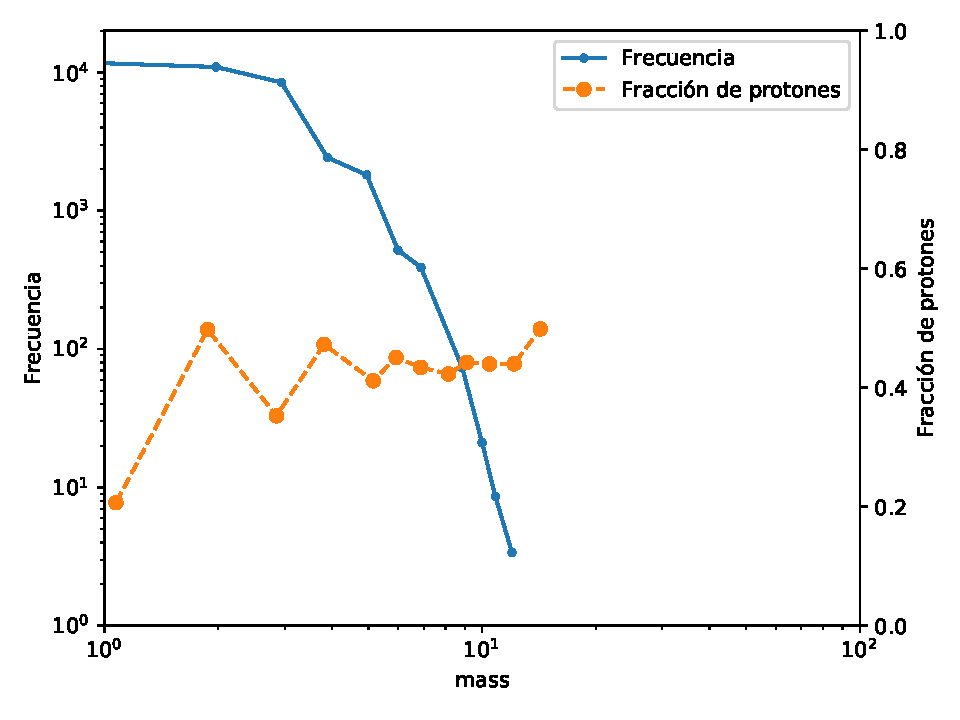
\includegraphics[width=\columnwidth]{fragmentacion/cluster_3e-2}
    \caption{$\eta = 0.03\,\text{fm/c}$}
    \label{subfig:3e-2}
  \end{subfigure}
  \caption{Distribución de masa de fragmentos.
    Las etiquetas aumentan junto a la velocidad de expansión.
    El sistema consiste de 11000 partículas con $x=0.4$ y densidad inicial $\rho_0 = 0.08\,\text{fm}^{-3}$}
  \label{fig:distribution}
\end{figure}

\section{Dependencia de la configuración con el potencial}

\begin{figure} \centering
  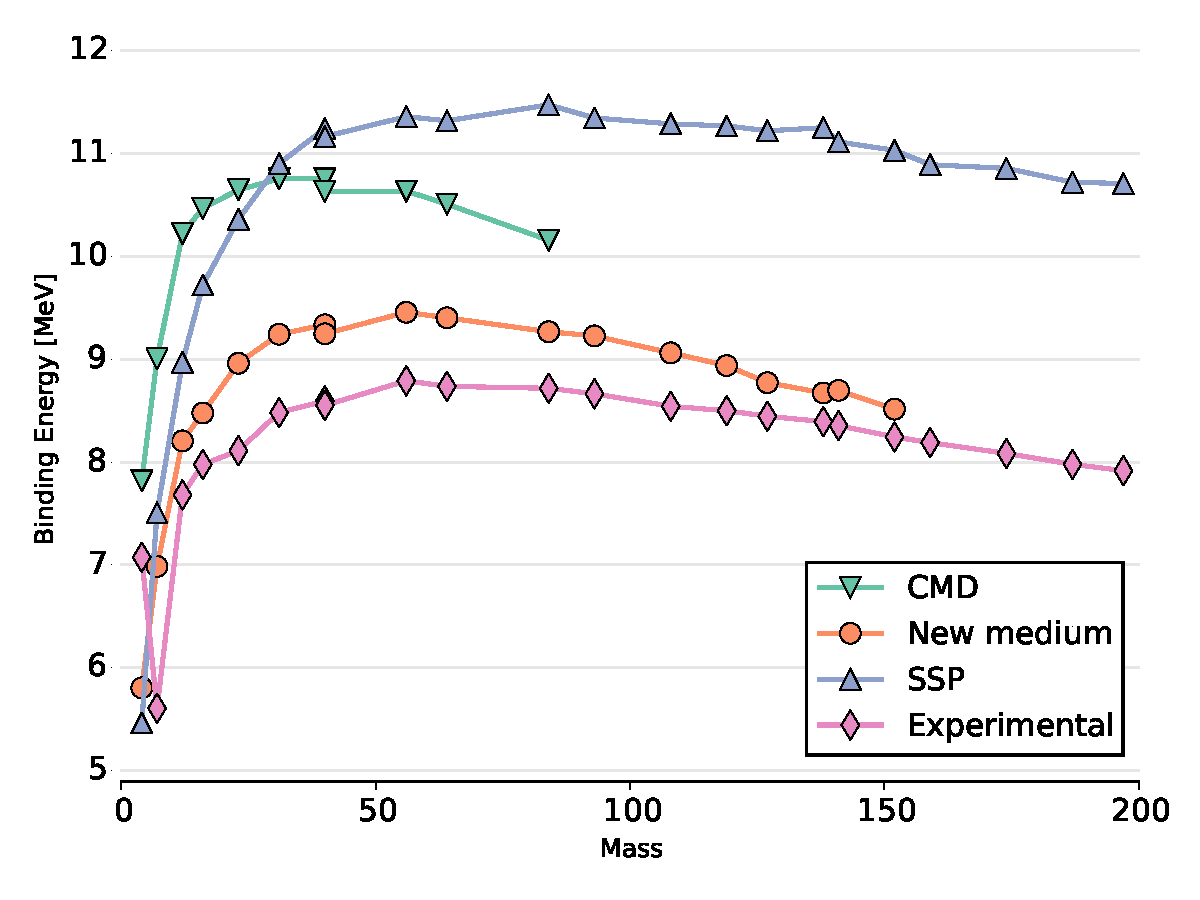
\includegraphics[width=0.7\columnwidth]{fragmentacion/binding}
  \caption{Energía de unión para las distintas parametrizaciones y datos experimentales.
    Podemos observar que las tres parametrizaciones reproducen cualitativamente el comportamiento de la energía de ligadura.}
  \label{fig:binding}
\end{figure}
La forma característica de la energía de unión para los núcleos terrestres puede reproducirse con varios modelos de interacción entre las partículas.
En la figura~\ref{fig:binding} observamos la energía de unión para tres potenciales distintos: \emph{CMD medium}, \emph{Simple Semiclassical Potential} y \emph{New Medium}, una parametrización inspirada en los potenciales de Pandharipande~\cite{akmal_equation_1998} pero con parámetros distintos.

\begin{figure*}
  \begin{subfigure}{.3\linewidth}
    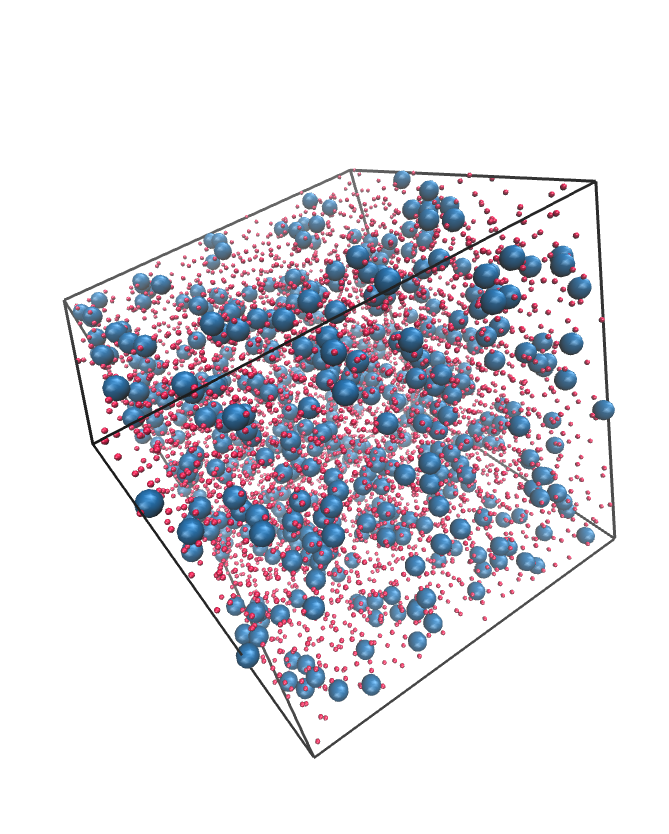
\includegraphics[width=\columnwidth]{fragmentacion/pregnocchi_med.png}
    \caption{CMD medium}
  \end{subfigure}
  \begin{subfigure}{.3\linewidth}
    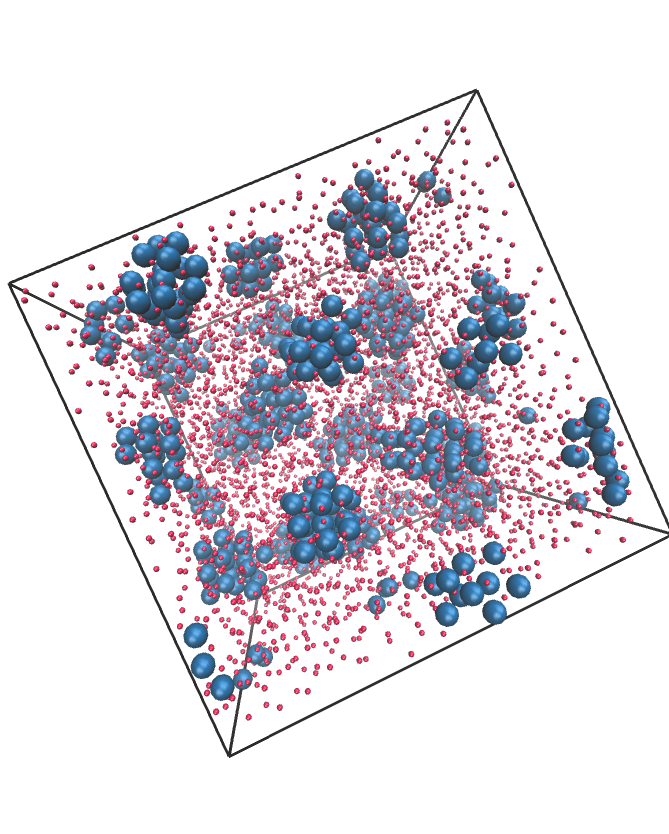
\includegraphics[width=\columnwidth]{fragmentacion/pregnocchi_newmed.png}
    \caption{New medium}
  \end{subfigure}
  \begin{subfigure}{.3\linewidth}
    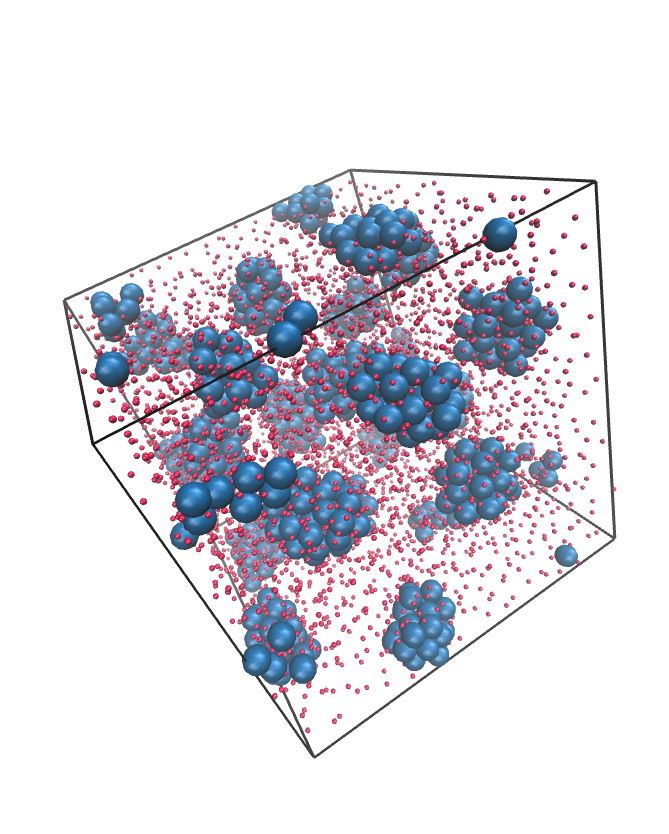
\includegraphics[width=\columnwidth]{fragmentacion/pregnocchi_horo.png}
    \caption{SSP}
  \end{subfigure}
  \caption{Imágenes de configuraciones para distintas parametrizaciones de la interacción nuclear, todas con las mismas condiciones termodinámicas: $x = 0.1$, $\rho = 0.05\,\text{fm}^{-3}$ y $T = 0.1\,\text{MeV}$.
    Las diferencias cualitativas entre el potencial tipo medio de CMD y las otras dos parametrizaciones (New Medium y SSP) son evidentes.
    Llamamos estas estructuras que aparecen en New Medium y SSP \emph{pregnocchi}.
    Para facilitar la identificación de la estructura de protones, los neutrones están representados por puntos muy pequeños comparados con los protones.}
\label{fig:x01_potentials}
\end{figure*}

\begin{figure*}
  \begin{subfigure}{.3\linewidth}
    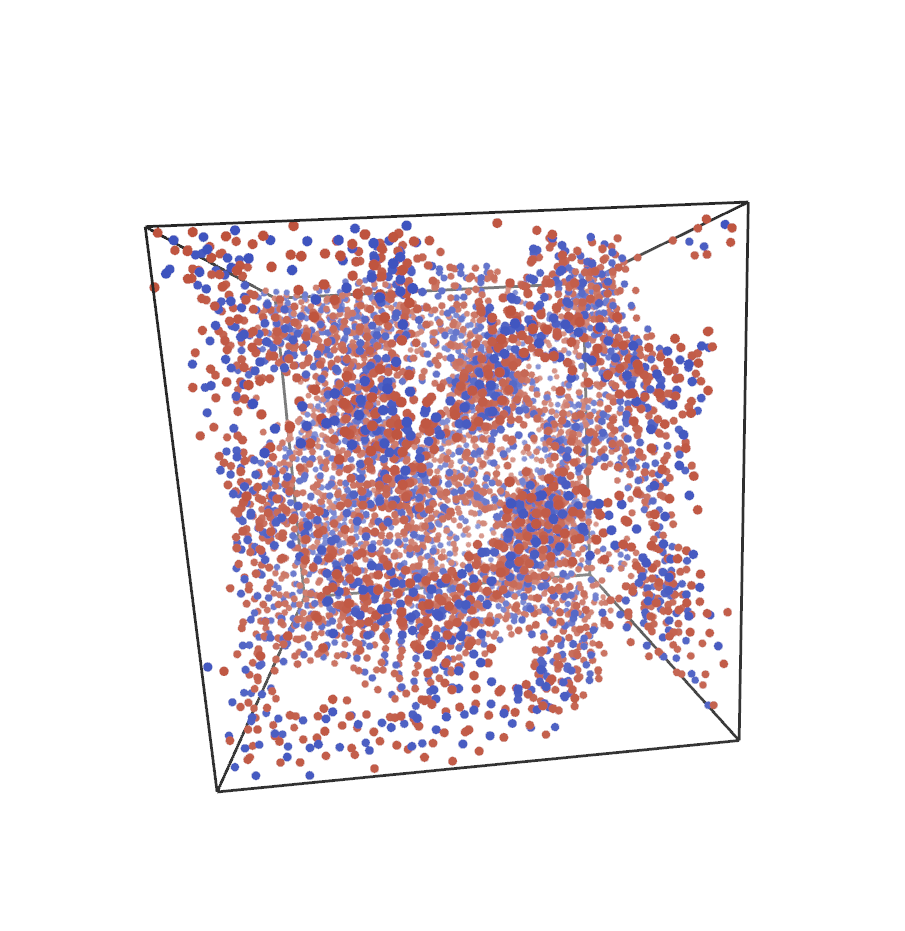
\includegraphics[width=\columnwidth]{fragmentacion/jungle_gym.png}
    \caption{Medium}
  \end{subfigure}
  \begin{subfigure}{.3\linewidth}
    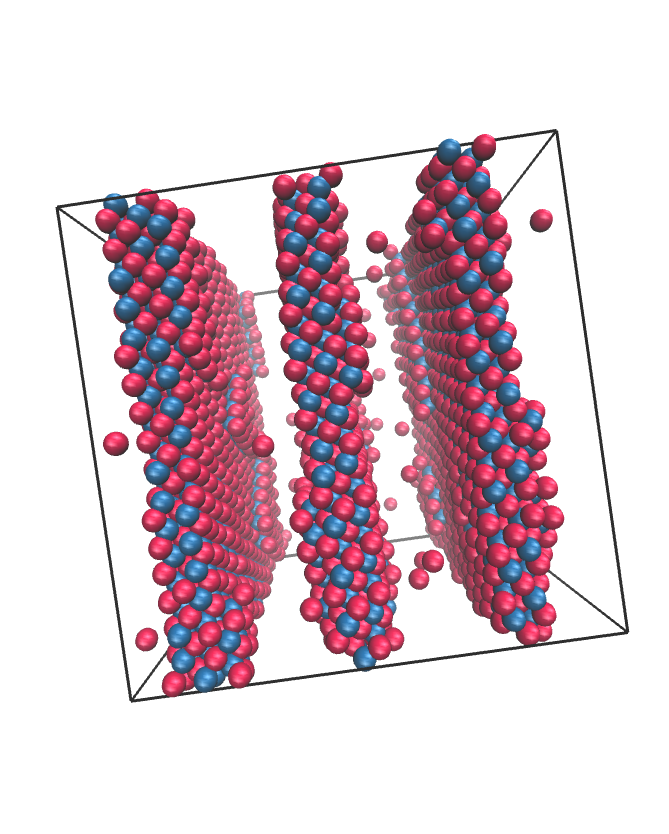
\includegraphics[width=\columnwidth]{fragmentacion/lasagna_newmed.png}
    \caption{New medium}
  \end{subfigure}
  \begin{subfigure}{.3\linewidth}
    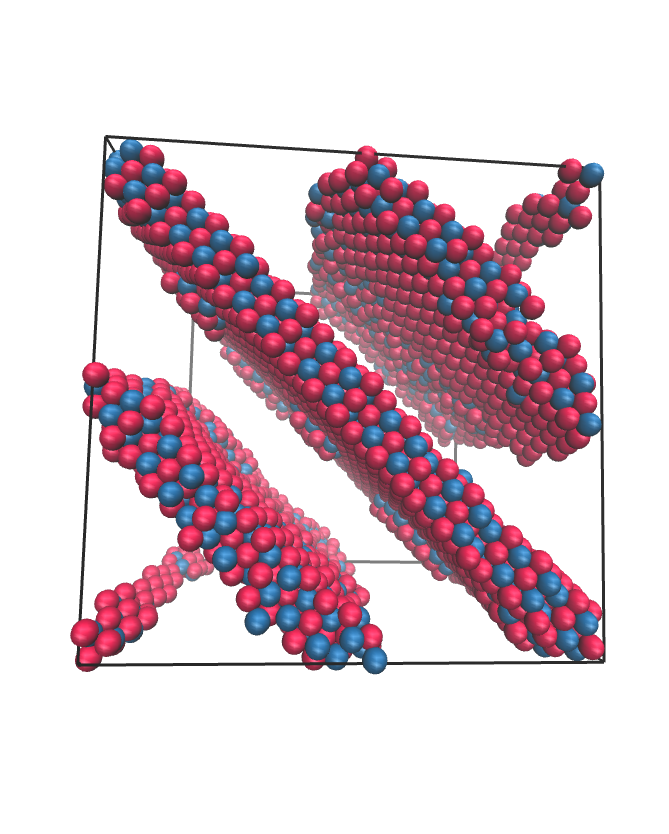
\includegraphics[width=\columnwidth]{fragmentacion/lasagna_horo.png}
    \caption{SSP}
  \end{subfigure}
  \caption{Imágenes de configuraciones para distintas parametrizaciones de la interacción nuclear, todas con las mismas condiciones termodinámicas: $x = 0.4$, $\rho = 0.05\,\text{fm}^{-3}$ y $T = 0.1\,\text{MeV}$.
    Las diferencias cualitativas entre el potencial tipo medio de CMD y las otras dos parametrizaciones (New Medium y SSP) son evidentes.
    Mientras que el potencial CMD muestra una estructura de tipo \emph{jungle gym}, tanto New Medium como SSP muestra \emph{lasagna} que son ligeramente diferentes entre sí.}
\label{fig:x04_potentials}
\end{figure*}


Estos distintos modelos de interacción resultan en distintas ecuaciones de estado y, en consecuencia, distintas distribuciones espaciales.
Para comparar, mostramos en la figura~\ref{fig:x01_potentials} distintas imágenes para los tres modelos estudiados: \emph{CMD medium}, \emph{New medium} y \emph{SSP}.
Estas estructuras son cercanas al estado fundamental, con temperatura muy baja ($T = 0.1\,\text{MeV}$), densidad $\rho = 0.05\,\text{fm}^{-3}$ y una fracción de protones de $x = 0.1$.
Las diferencias son notorias: mientras que el potencial \emph{CMD medium} no tienen ninguna estructura identificable, \emph{New medium} y \emph{SSP} muestran claramente aglomeraciones de protones (debido a la interacción atractiva que median los neutrones) embebidos en un \emph{mar de neutrones}.
Esta estructura la llamaremos \emph{pre-gnocchi}.
Esta es la primera vez que se observa este tipo de estructuras, y es también una muy interesante diferencia \emph{cualitativa} observadas entre parametrizaciones de la ecuación de estado.

Para comparar los potenciales en otra configuración, mostramos en la figura~\ref{fig:x04_potentials} distintas imágenes para los tres modelos que estudiamos: \emph{CMD medium}, \emph{New medium} y \emph{SSP}.
Estas estructuras son cercanas al estado fundamental, con temperatura muy baja ($T = 0.1\,\text{MeV}$), densidad $\rho = 0.05\,\text{fm}^{-3}$ y una fracción de protones de $x = 0.4$.

\section{Distribución Asintótica de Masas}
Cuando el sistema se expande, la estructura se parte en fragmentos finitos.
Para tiempos suficientemente largos, estos fragmentos permanecen estables, ya que no interactúan entre sí y se han desexcitado por emisión de partículas.
Llamaremos a estos ``fragmentos asintóticos''.

Expandimos distintas configuraciones iniciales con el modelo \emph{New medium} para encontrar la distribución asintótica de masas.
Como primer ejemplo, mostramos en la figura~\ref{fig:asymp_preg} la distribución asintótica de masas (calculada con el algoritmo MSTE) para $x = 0.1$, $\rho = 0.05\,\text{fm}^{-3}$ y $T = 0.8\,\text{MeV}$ para dos velocidades de expansión: \emph{rápida} ($\dot{\eta} = 0.01\,\text{c/fm}$)y \emph{lenta} ($\dot{\eta} = 0.0001\,\text{c/fm}$)
Podemos ver aquí que la expansión lenta permite la existencia de fragmentos con masa de hasta 60 (20 de los cuales son protones) mientras que la expansión rápida produce fragmentos más pequeños de hasta 20 (6 protones).
Este comportamiento es esperado, ya que cuanto más rápida la expansión, mayor la energía de excitación que se le agrega al sistema.
En consecuencia, una expansión más rápida debería romper fragmentos que, de otro modo, serían estables.
Un comportamiento similar se puede ver en la figura~\ref{fig:asymp_las}, donde expandimos el sistema para $x = 0.4$, $\rho = 0.05\,\text{fm}^{-3}$ y $T = 0.1\,\text{MeV}$ para las mismas velocidades de expansión rápida y lenta.
Otra característica relevante de la distribución asintótica de masas (que no se muestra en la figura debido a limitaciones de escala) es que la expansión rápida tiene una fracción no despreciable de neutrones sueltos (cerca del $4\%$) mientras que la expansión lenta presenta muy pocos ($0.1\%$).

\begin{figure}[h]
  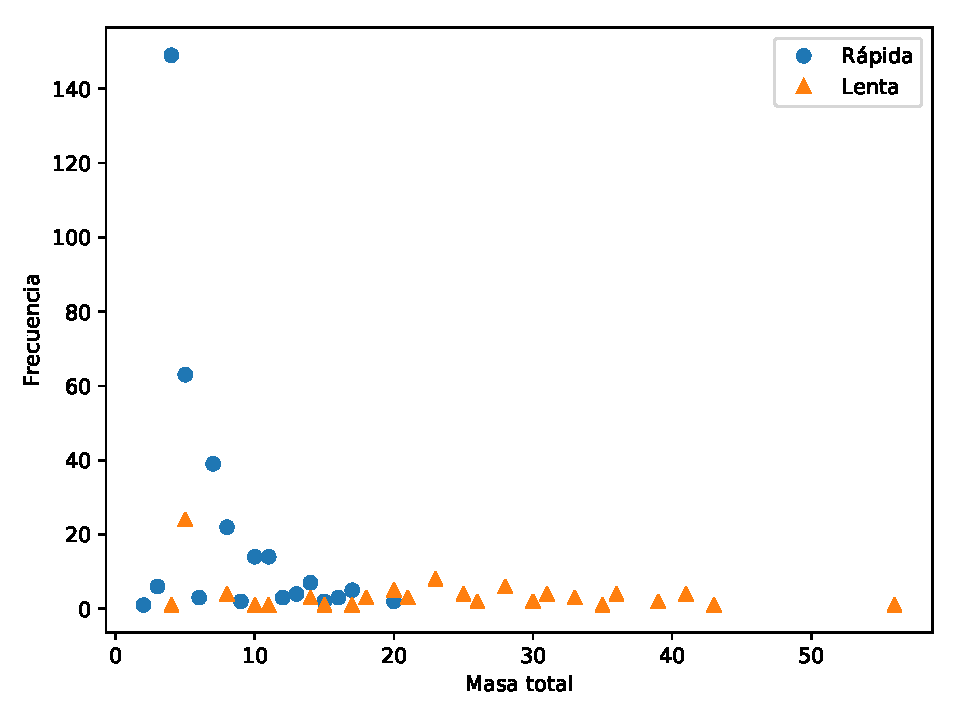
\includegraphics[width=0.8\columnwidth]{fragmentacion/pregnocchi}
  \caption{Distribución asintótica de masas para $x = 0.1$, $\rho = 0.05\,\text{fm}^{-3}$ y $T = 0.8\,\text{MeV}$ y dos velocidades de expansión distintas: \emph{rápida} $\dot{\eta} = 0.01\,\text{c/fm}$ y \emph{lenta} $\dot{\eta} = 0.0001\,\text{c/fm}$.}
\label{fig:asymp_preg}
\end{figure}

\begin{figure}[h]
  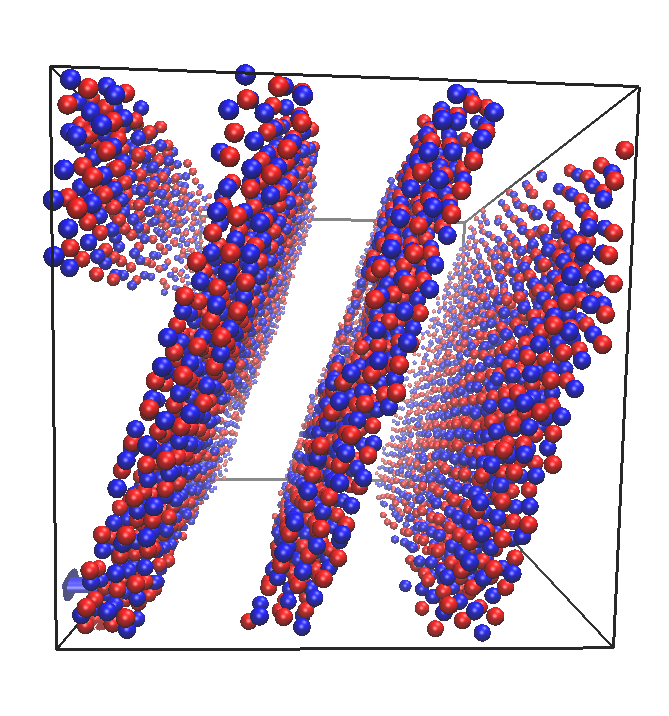
\includegraphics[width=0.8\columnwidth]{fragmentacion/lasagna}
  \caption{Distribución asintótica de masas para $x = 0.4$, $\rho = 0.05\,\text{fm}^{-3}$ y $T = 0.1\,\text{MeV}$ y dos velocidades de expansión distintas: \emph{rápida} $\dot{\eta} = 0.01\,\text{c/fm}$ y \emph{lenta} $\dot{\eta} = 0.0001\,\text{c/fm}$.}
\label{fig:asymp_las}
\end{figure}


\section{Formación de fragmentos}
\newcommand{\tabfig}[1]{\includegraphics[width=0.25\linewidth]{fragmentacion/#1}}

\begin{table*}
  \centering
  \begin{tabular}{cccc}
    \toprule
    & Lasagna (expansión rápida) & Lasagna (expansión lenta) & Pregnocchi \\
    \midrule
    $\rho = 0.05\,\text{fm}^{-3}$ & \tabfig{las_fast_0} & \tabfig{las_slow_0} & \tabfig{pregnocchi_0} \\
    $\rho = 0.0001\,\text{fm}^{-3}$ & \tabfig{las_fast_100} & \tabfig{las_slow_100} & \tabfig{pregnocchi_100} \\
    $\rho = 0.00003\,\text{fm}^{-3}$ & \tabfig{las_fast_400} & \tabfig{las_slow_400} & \tabfig{pregnocchi_400} \\
    \bottomrule
  \end{tabular}
  \caption{Tres distintas expansiones de materia de estrellas de neutrones: Lasagna (expansión rápida): $x = 0.4$, $\dot{\eta} = 0.01\text{c/fm}$, $T = 0.8\,\text{MeV}$;
    Lasagna (expansión lenta): $x = 0.4$, $\dot{\eta} = 0.0001\text{c/fm}$, $T = 0.8\,\text{MeV}$;
    Pregnocchi: $x = 0.1$, $\dot{\eta} = 0.0001\text{c/fm}$, $T = 0.1\,\text{MeV}$}
\label{tbl:expansion}
\end{table*}

Ahora nos centramos en el análisis de algunos ejemplos de la evolución del sistema en el tiempo: cuándo y cómo se forman los fragmentos asintóticos.
Tomemos primero la expansión del sistema con $x = 0.4$, $\rho = 0.05\,\text{fm}^{-3}$ y $T = 0.5\,\text{MeV}$.
Mostramos en las primeras dos columnas de la tabla~\ref{tbl:expansion} los estados iniciales y asintótico con la expansión rápida y lenta para la \emph{lasagna}.
Mientras que la condición inicial es un cluster infinito, en el régimen asintótico tenemos una distribución de fragmentos con muchos fragmentos finitos.
Es interesante notar que la expansión rápida se parece a una fractura mecánica, en la que los fragmentos se forman dentro de cada hoja de la \emph{lasagna}, mientras que la expansión lenta parece más una expansión térmica en la que el sistema asintótico pierde todo tipo de similitud con la estructura original.
Los fragmentos se parten en muchos porque su tamaño tan grande no puede soportar la energía asociada con la expansión del sistema.

Un escenario muy interesante es la expansión del sistema con baja fracción de protones: $x = 0.1$, $\rho = 0.05\,\text{fm}^{-3}$ y $T = 0.1\,\text{MeV}$.
En la tercera columna de la tabla~\ref{tbl:expansion} mostramos tanto la condición inicial como la configuración asintótica para $\dot{\eta} = 0.0001\,\text{c/fm}$. \todo[inline]{Es como supernova?}

A diferencia del escenario anterior, aquí hay una clara estructura de protones: los fragmentos existen desde el comienzo, inmersos en un mar de neutrones.
Pueden ser identificados visualmente si dibujamos los protones con un tamaño mucho mayor que el de los neutrones, como se ve en este conjunto de figuras.
A medida que el sistema se expande, se modifica.
Esto genera la siguiente pregunta: ¿la distribución de fragmentos se modifica sustancialmente?
La respuesta a esta pregunta requiere de un análisis profundo de la evolución temporal de la distribución de fragmentos, y no podemos confiar en una inspección visual; necesitamos usar algoritmos de reconocimiento de fragmentos.
Este tipo de análisis ha sido realizado previamente para sistemas finitos, por ejemplo en Ref.~\cite{dorso_fluctuation_1994, strachan_fragment_1997}.
En la figura~\ref{fig:mste_pregnocchi} mostramos las configuraciones iniciales y final con el algoritmo de MSTE.\@
Podemos notar que la distribución de clusters cambia radicalmente en ambos aspectos: el tamaño y la fracción de protones.
El cambio en la fracción de protones es de esperar ya que, a medida que el sistema se expande, menos neutrones están en el rango del fragmento de protones.
Sin embargo, este efecto solo no explica el cambio de tamaño: mientras que la condición inicial muestra un fragmento de hasta 80 protones, el fragmento más grande de la distribución asintótica tiene aproximadamente 30 protones.
¿Se rompió un cluster mientras el sistema se expandía?

\begin{figure}
  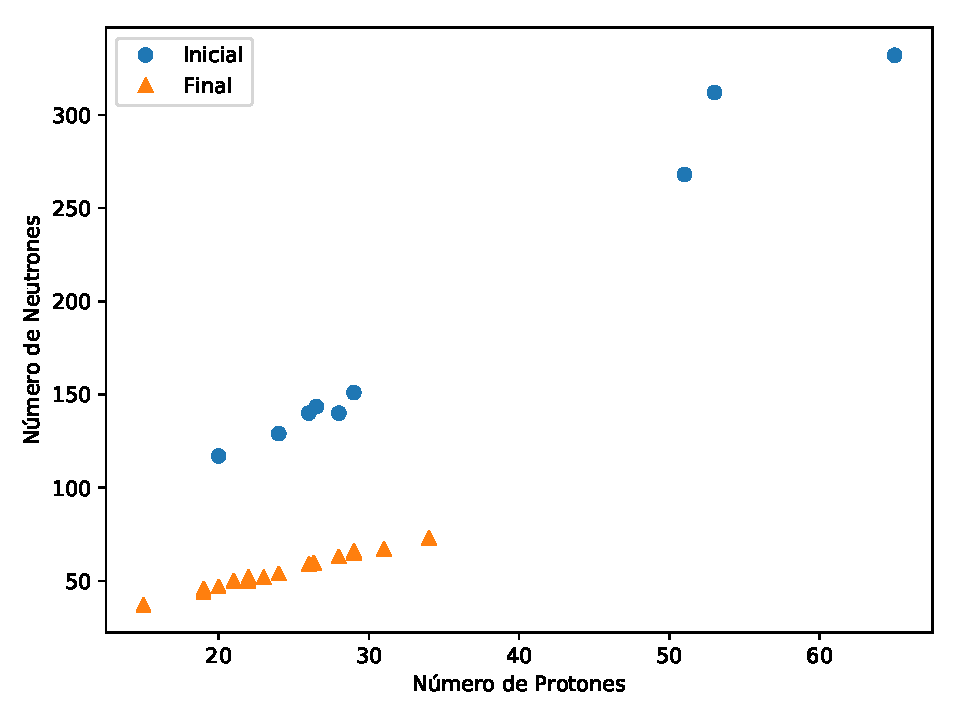
\includegraphics[width=0.8\columnwidth]{fragmentacion/mste}
  \caption{Distribución asintótica e inicial de masas para un sistema con $x = 0.1$, $\rho = 0.05\,\text{fm}^{-3}$ y $T = 0.1\,\text{MeV}$, para una expansión lenta ($\dot{\eta} = 0.0001\text{c/fm}$), con el algoritmo de reconocimiento MSTE.}
\label{fig:mste_pregnocchi}
\end{figure}

\begin{figure}
  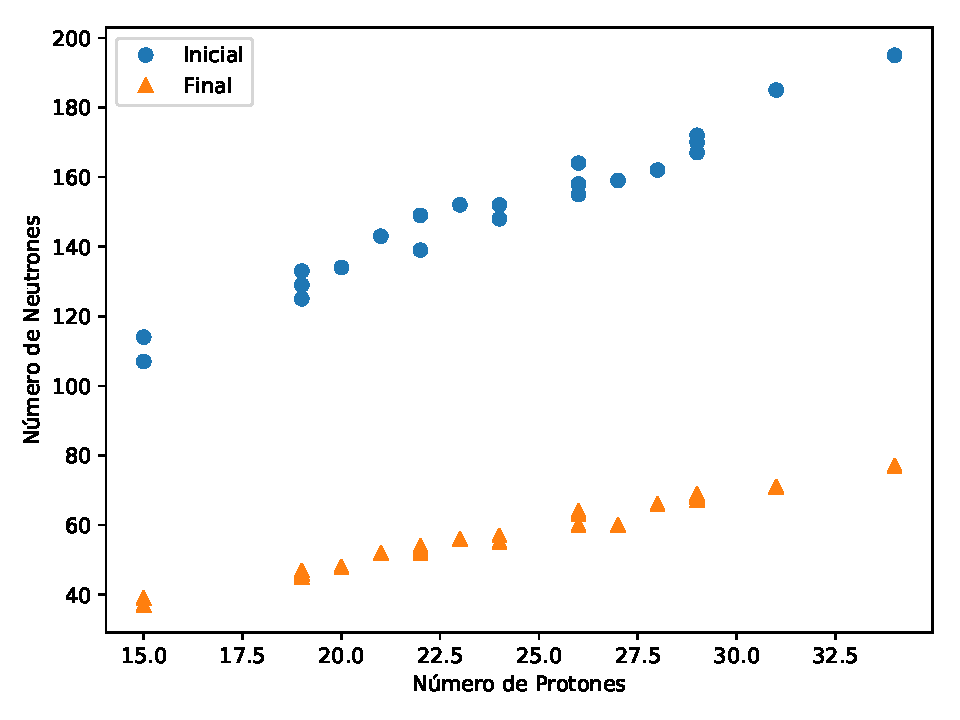
\includegraphics[width=0.8\columnwidth]{fragmentacion/mst_nube}
  \caption{Distribución asintótica e inicial de masas para un sistema con $x = 0.1$, $\rho = 0.05\,\text{fm}^{-3}$ y $T = 0.1\,\text{MeV}$, para una expansión lenta ($\dot{\eta} = 0.0001\text{c/fm}$), con el algoritmo de reconocimiento MST para protones.}
\label{fig:mst_pregnocchi}
\end{figure}

Para analizar esto, estudiamos la distribución con el algoritmo MST aplicado a los protones solos, mostrados en la figura~\ref{fig:mst_pregnocchi}.
De acuerdo a esta figura, vemos que la distribución de fragmentos de los protones no cambió sustancialmente (sólo un cluster de protones se rompió) y, efectivamente, el fragmento más grande tiene 32 protones.
¿Qué tipo de resultados se obtienen del algoritmo ECRA, teóricamente más sólido?
En la figura~\ref{fig:ecra_pregnocchi} mostramos que de hecho el algoritmo ECRA-BFM dio buenos resultados, e identifica los pre-clusters adecuadamente, incluso encontrando el fragmento que se rompió.

\begin{figure}
  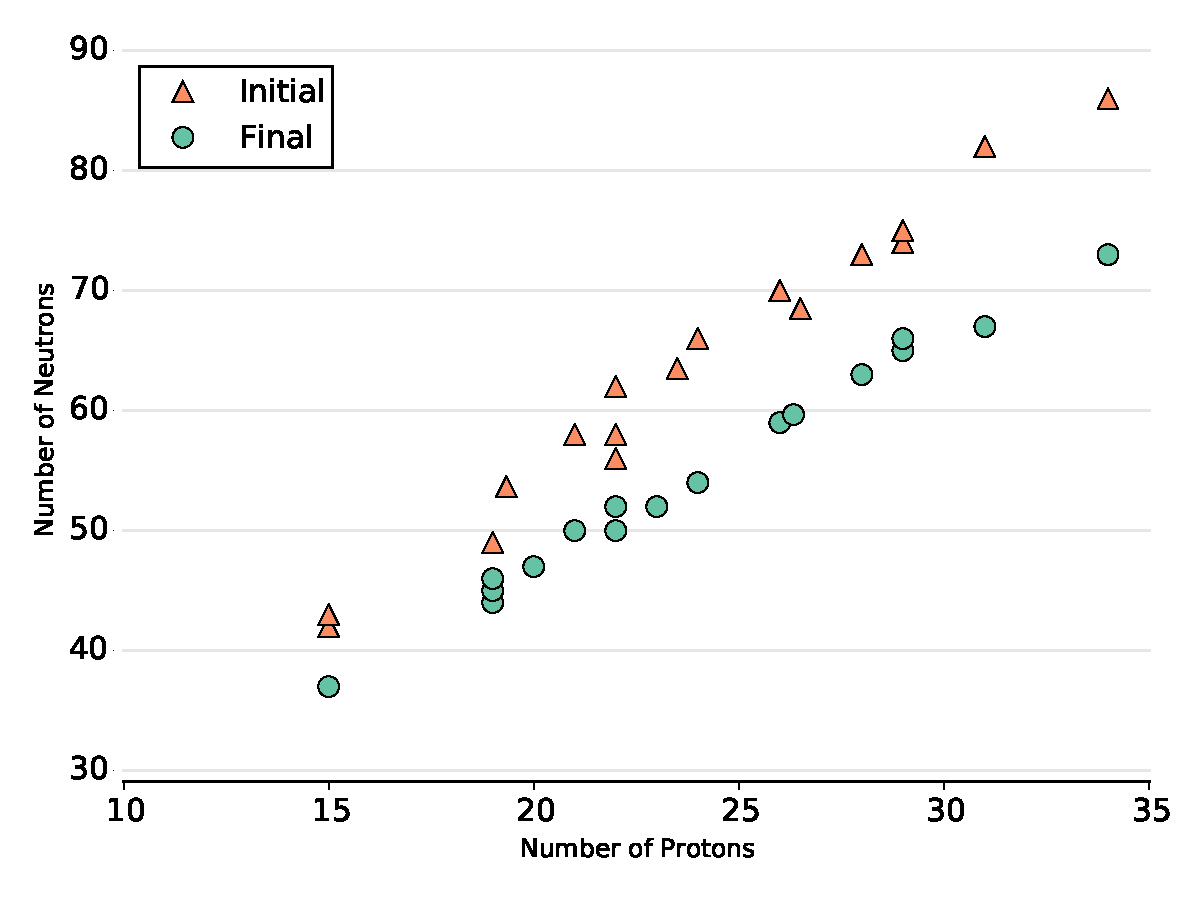
\includegraphics[width=0.8\columnwidth]{fragmentacion/ecra}
  \caption{Distribución asintótica e inicial de masas para un sistema con $x = 0.1$, $\rho = 0.05\,\text{fm}^{-3}$ y $T = 0.1\,\text{MeV}$, para una expansión lenta ($\dot{\eta} = 0.0001\text{c/fm}$), con el algoritmo de reconocimiento ECRA. Al comparar con la figura~\ref{fig:mst_pregnocchi}, notar la diferencia de escalas en el eje $y$.}
\label{fig:ecra_pregnocchi}
\end{figure}

Con estos resultados en mente, utilizamos tres herramientas para el reconocimiento de fragmentos: MSTE, ECRA y MSTpC.
MSTE y ECRA son los algoritmos ya descritos, mientras que MSTpC es el algoritmo de MST sobre protones con la nube de neutrones que están cerca de cada cluster MST.\@
En la figura~\ref{fig:lm_pre} mostramos la evolución del tamaño del fragmento más grande para las etapas iniciales de la evolución para los tres reconocedores de fragmentos: MSTE, MSTpC y ECRA.\@
La figura muestra que el fragmento ECRA se estabiliza rápido y se mantiene relativamente estable, mientras que los otros dos algoritmos resultan en fragmentos que son siempre más grandes que los ECRA y se estabilizan más lentamente.
También es interesante notar que el fragmento MSTpC comienza con alrededor de 100 neutrones más que el fragmento ECRA correspondiente, lo que implica que el fragmento de ECRA está en un ambiente muy rico en neutrones.
Esta situación sugiere que existe la posibilidad del \emph{r-process}, a diferencia de cálculos anteriores~\cite{caplan_pasta_2015}.

Por el otro lado, en la expansión de la estructura de \emph{lasagna}, ninguno de los algoritmos reconocedores de fragmentos identifican fragmentos en tiempos muy tempranos de la evolución (ver figura~\ref{fig:lm_las}).
En esta etapa hay un fragmento muy grande (que, de hecho, es infinito).
De cualquier modo, el análisis de ECRA muestra que este fragmento se parte tempranamente en muchos fragmentos y, como resultado, la masas del fragmento más grande decrece drásticamente con el tiempo.
Es interesante notar que, a diferencia de los \emph{pregnocchi}, en este caso el algoritmo MSTpC es el que más tiempo toma para identificar que el fragmento infinito se parte.
Esto muestra que el algoritmo de ECRA es además más versátil para estudiar la formación temprana de fragmentos.
También es interesante notar (no se muestra en las figuras) que la fracción de protones $x$ de estos fragmentos es relativamente estable para el algoritmo ECRA, mientras que los otros dos resultan en una fracción de protones que decae monótonamente con el tiempo.

\begin{figure}[H]  \centering
  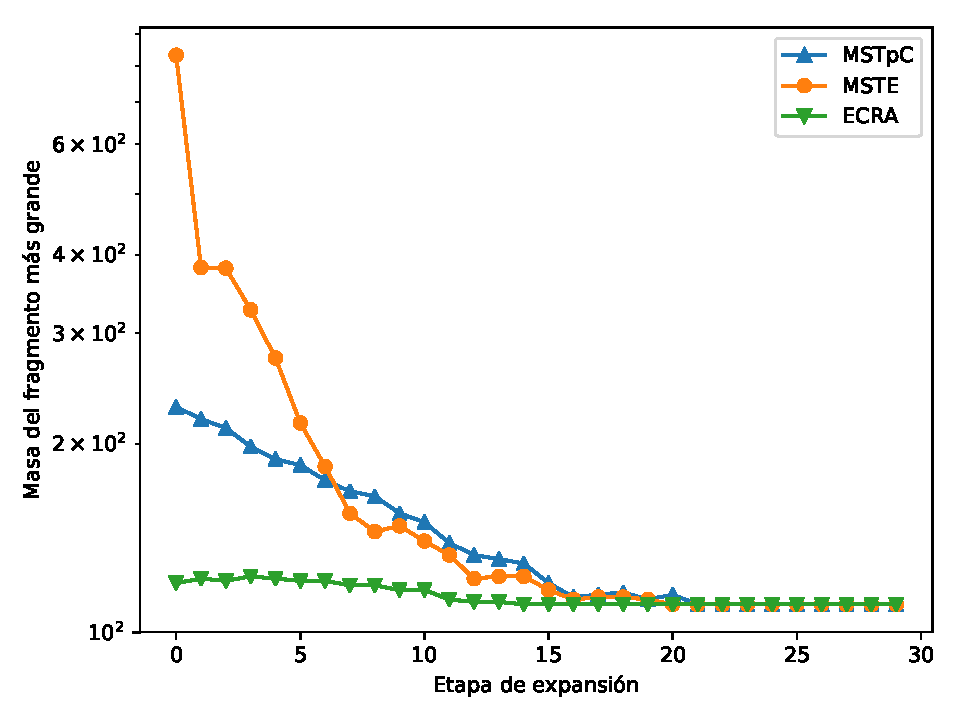
\includegraphics[width=0.8\columnwidth]{fragmentacion/lm_pre}
  \caption{Masa del fragmento más grande para MSTE, MSTpC y ECRA para las etapas iniciales de la evolución, para la configuración \emph{pre-gnocchi}.
    Se puede observar que el fragmento de ECRA se mantiene relativamente estable y se estabiliza rápidamente, mientras que los otros dos algoritmos resultan en fragmentos que son siempre más grandes y tardan más en estabilizarse.}
\label{fig:lm_pre}
\end{figure}

\begin{figure}[H]  \centering
  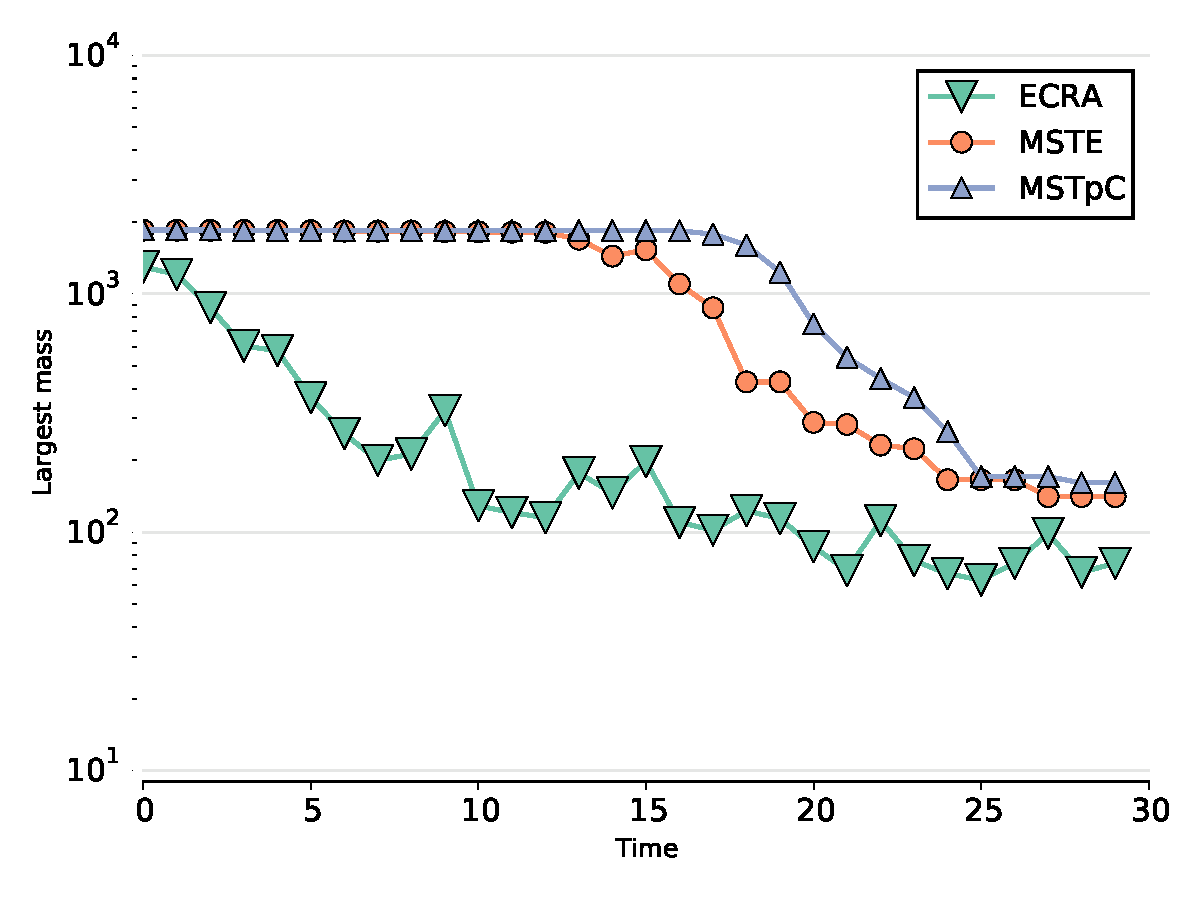
\includegraphics[width=0.8\columnwidth]{fragmentacion/lm_las}
  \caption{Masa del fragmento más grande para MSTE, MSTpC y ECRA para las etapas iniciales de la evolución, para la configuración \emph{lasagna}.
    Aquí se puede notar que, como en el caso anterior, el algoritmo ECRA reconoce la fractura del fragmento infinito muy tempranamente.
    En el régimen asintótico (por tiempos muy largos, no se muestra en las figuras) estos tres algoritmos dan los mismos resultados.}
\label{fig:lm_las}
\end{figure}


\section{Conclusiones}\label{sc:conc}


Desarrollamos experimentos numéricos de sistemas expandidos homogéneamente  y, para analizar la estructura del sistema en función del tiempo, desarrollamos una herramienta basada en análisis de grafos para identificar fragmentos infinitos para cualquier tipo de fragmentos aditivos.
Una vez que esta formalismo fue aplicado a las simulaciones mencionadas, pudimos identificar la región en la que se da una distribución de fragmentos de tipo ley de potencias.
Esta distribución tiene formas desde U-shaped hasta decaimiento exponencial.

También estudiamos las propiedades estructurales de la corteza de estrellas de neutrones a través de tres potenciales distintos.
Estos potenciales involucran un término nuclear escogido para reproducir energías de ligadura y compresibilidad de la materia nuclear, sumado a la interacción de Coulomb.
Para analizar las estructuras que se forman utilizamos cuatro tipos distintos de algoritmos reconocedores de fragmentos: MST, MSTE, MSTpC y ECRA-BFM.
Con estos algoritmos encontramos que de los tres potenciales, dos de ellos (New Medium y SSP) desarrollaron una estructura nueva para bajas fracciones de protones que llamamos \emph{pregnocchi}.
Esta estructura consiste en agregados de protones formados por la mediación del término atractivo $V_{np}$ del potencial que resistieron la expansión.

También analizamos la expansión de materia rica en neutrones infinita descripta a través del modelo del pequeño big bang.
Mostramos que, en general, la identificación adecuada de la estructura depende mucho del algoritmo escogido, siendo ECRA y MSTpC los más adecuados para encontrar las estructuras y ECRA el más estable.
Este enfoque, combinado con distintos algoritmos reconocedores de fragmentos, nos permitió identificar la dinámica de la formación de fragmentos.
El estado asintóticos mostró una alta dependencia con la velocidad de expansión, tanto en la distribución de masa como en la distribución espacial de los fragmentos: para velocidades suficientemente altas, la expansión era similar a una \emph{fractura mecánica}, donde la distribución espacial estaba altamente correlacionada con el estado original.
Sin embargo, para velocidades más bajas, la expansión era una \emph{expansión térmica}, en la que el estado asintótico era relativamente homogéneo.
Los fragmentos formados en la expansión más lenta eran mucho más grandes que los formados en la expansión rápida.
Un análisis cuidadoso de la dinámica de formación de fragmentos mostró que se formaron muy temprano en la expansión.
En particular, la novedosa estructura que llamamos \emph{pregnocchi}
es de considerable relevancia, ya que de acuerdo al análisis de ECRA
estos agregados preexistentes evolucionan en una nube de neutrones,
resultando en configuraciones en las que el \emph{r-process} se puede
desarrollar.
%  LocalWords:  process
